\subsection{Parameterization Discussion} \label{sub_sec:param_discussion}

%----------- SIMPLIFICATIONS -----------%

\subsubsection{Simplifications}

Certain aspects of the parameterization were simplified.
First, some parts were simplified to single variable parameterization problems, whereas in reality they may have multiple changing variables.
For example, the belt system calculation was simplified by setting a constant belt pitch, belt width and belt thickness to reduce from volumetric parameterization to single variable parameterization. The only dimension that is calculated is the pulley diameter. The length of the belt is geometrically set by other parameters such as the length of the thigh.

When calculating the load carried by each leg, the position of each foot must be approximated to use the matrix approach as done in Section 4.3 of the Modelling report. This approach calculates higher normal forces for one foot as the centre of mass is not evenly distributed, compared to dividing the mass by 3 (loosely approximating 3 legs making contact with the ground).
However, the position of the feet are not re-calculated in the program, this was due to time constraints, resulting in a simplification of the method to a ratio approach.

The ratio between the leg linkage lengths, as defined in Section 3.4 of the Analysis Report, are constant and were determined experimentally as shown in Appendix \ref{app_sub:linkages}. When leg reaches in $x$ and $y$ are passed by the GUI, they are compared to reference leg reaches and scaled accordingly. If the desired $x$ reach is half the reference one, then the linkage lengths will also be halved. Since the leg linkages are related by ratios, this causes the $y$ reach to scale with the $x$ reach, in that it may be larger than the required value. A more ideal approach would have been to independently vary the lengths of the linkages to produce a configuration that more closely matches the given $x$ and $y$ reach.

The bellow was not parameterized as per the equations presented in Section 4.9 of the Analysis Report. The construction of the part in SolidWorks was limited in that it was not possible to change the number and size of the folds to match the equations. Thus, only the diameters of the bellow scale with the robot. The change in those values also modifies the length of the folds consequently.
The thigh angle varies from $0^{\circ}$ to $28^{\circ}$ from horizontal, and the tibia angle varies from $-22.5^{\circ}$ to $22.5^{\circ}$ from the thigh.
These constraints are to ensure the bellow does not stretch too far in either direction.

The solar cells were not added in the parameterized assembly due to time constraints and the complexity of positioning parts on a non-rectangular area. The number of solar cells is calculated and is output into the Matlab Command Window.

The sleeve bearings were not parameterized, as the results of the calculations gave small and sometimes unrealistic lengths. These lengths did not ensure enough penetration into the hip plates or hip brackets for a stable assembly. As a simplification, the length was set to a larger constant value. As the width of the hip plates and hip brackets is constant, the bearings were made to match that width. Their diameters scale with that of the shafts.

To ensure that the steps on the shafts were sufficiently large to properly position components axially, the difference between the small and large diameter of the shafts was always set to 4 mm.

The foot assembly was simplified by only using the tibia tube diameter as a parameterization input, and maintaining a total assembly height of $100\text{mm}$. This results in a constant radius for the spherical portion of the silicone sock. However, when the size of the tibia tube changes, the shape of the silicone sock changes. When the tube is larger, the silicone becomes thin in some areas and can cause the parameterization to fail once the tube surpasses the set radius. More parameterized dimensions should be added to ensure the silicone sock keeps its required shape, regardless of how large the tibia tube becomes.

Traditional \texttt{for} loops were used for most of the components; a single variable is manipulated in the loop to find an acceptable solution, while all other variables are set as a constant or as ratios of others.
The usage of vectorized loops (as shown in Appendix \ref{app_ssub:vectorization_spring}) for the springs simplified parameterizing multiple variables simultaneously. This approach could have also been applied to other parts whose geometry suffered due to variables that were set as constants or ratios.

The stability analysis summarized in Section 3.3 of the Analysis Report was not performed due to time constraints. The centre of mass of the robot would have needed to be computed, which would have been a long process due to the large amount of parts in the robot. Components were positioned in a manner to provide as much stability as possible, as per observations made in the previous stability analysis. However, the stability of the robot on the required slope was not verified.

As mentioned in the Analysis Report, the tensioner torsion spring was not parameterized as the equations were never fully developed.

The electronics were not positioned in the parameterized assembly, as the internal dimensions vary significantly between different leg reaches and litter box dimensions. There is no simple way of placing them that would satisfy all possible robot configurations. A comparison of a small and large robot with the same litter size is shown in Figure \ref{fig:elec}. The small robot has quite a bit of available space for the electronics in between the front and back legs, however the large robot would require more thought and analysis to ensure that the electronics do not interfere with the legs. 

\begin{figure}[H]
    \centering
    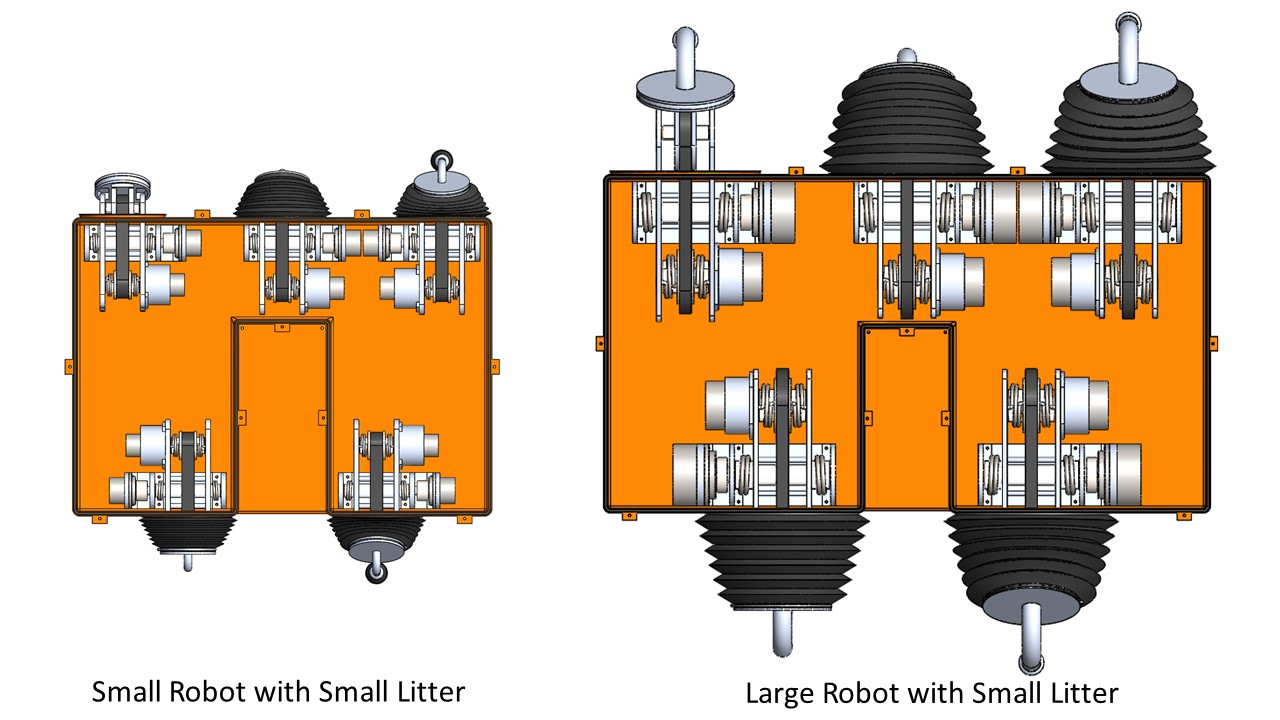
\includegraphics[width=0.9\textwidth]{3_Parametrization/img/ElectronicsA.jpg}
    \caption{Comparison of available areas for electronics in two robot configurations}
    \label{fig:elec}
\end{figure}

The torsion spring programming was also simplified slightly. The selection method should verify the shaft and pulley diameters to ensure the spring does not interfere with other components. However this method could not be properly integrated into the programming.


%----------- THINGS WE CONSTRAINED SO THEY WOULD NOT BREAK -----------%

\subsubsection{Constrained Parts} \label{ssub_sec:constrained_parts}

Some parts deviate from their parameterization loop if certain conditions are met.
If the motors are larger than the Harmonic Drives, their mounting bolts start interfering with the Harmonic Drive mounting bolts.
Since the motors scale in size faster than the Harmonic Drives, this occurs at the upper end of the leg reach.
To counteract this, the motor outer diameter and mounting diameter are limited to that of the Harmonic Drive.
In reality, some design changes would need to be made. A different motor or additional gearbox such as a single stage reducer could be used. Another option would be to modify the design of the adaptor onto which the motor and harmonic drive are attached.

All of the keyed components such as the pulley, hip plates and shaft collars were set to a fixed width equal to the width of the component they are in. However, as the torques in the legs increase, some of the keys require a larger length than is available in order to meet their safety factor (this is printed in the command window if it is the case). 
This would realistically be resolved by increasing the width of the component by adding a hub, or using a higher-strength material for the key.

When the desired $x$ and $y$ reach of the leg become too small and litter mass too large, the tibia tube interferes with the tibia holder. This is due to the tibia tube diameter increase with the robot mass. The mass also makes the torsion springs wider, increasing the shaft diameter and consequently the bellow and tibia holder diameters. The parameterization inputs were limited to ranges that avoid collisions between these parts.


%----------- NOVEL DEVELOPMENTS -----------%

\subsubsection{Additional Parameters and Analysis}

Many geometric aspects of the assembly were not considered in the Modelling and Analysis Reports.
The hip brackets connect the hip plates to the base plate and chassis. Their height had to be parameterized to ensure the leg would not hit the chassis bottom during movement. It was determined as a function of the maximum hip angle, diameters of the hip and knee adaptors, and dimensions of the hip plates.
The distance between the knee control shaft and hip control shaft on the hip plates was also calculated to avoid interference between the knee adapter and the hip brackets.
Another new geometrical relation was added for the radius of the bent portion of the tibia tube. As mentioned in Section 4.2.6 of the Analysis Report, no precise method could be developed to properly calculate the safety factor of the tube bend.  The parameterization was thus set to always be the maximum possible radius, so as to increase manufacturability.

In some cases, the performed parameterization was unnecessary.
The spring parameterization minimizes the number of turns and, within the chosen operating range, always gives 2; this variable could have been set as constant.
The fasteners were found to also always give an acceptable safety factor for diameters as low as M2s, even at the upper end of the parameterization input range; the parameterization for them could have been removed entirely.